
\chapter{Problem Description \& Serial Implementation}

\section{Problem Description}

Finding the longest common sub-sequence (LCS) between a set of two or more sequences (or strings) is a longstanding problem in computer science with many practical implications. It finds use, along with other sub-sequence problems, in applications where the differences between sequences are important, including linguistics, genomics and version-control software \cite{survey}.

In order to present the problem unambiguously, it is important to define several core terms:
\vspace{-1em}
\begin{itemize}
    \item Sequence: a contiguous series of symbols or characters. For example "$hello,world$" would be considered a single sequence.
    \item Sub-sequence: a collection of (not necessarily contiguous) characters from an existing sequence. The characters in the sub-sequence must occur in the same order as in the sequence it is derived from. For example "$howd$" is a sub-sequence of "$hello,world$", but "$hwod$" is not.
\end{itemize}

These distinctions are particularly vital in differentiating between the LCS problem and the similarly named, though very different Longest Common Sub-String problem, which requires the elements of the sub-sequence to occur contiguously in the original sequence.

The longest common sub-sequence is not limited to being performed between two sequences, and can easily be generalised to any number of strings, however this analysis focuses solely on LCS comparisons between pairs of sequences.

\section{Implementation} 
A wide variety of solutions to the LCS problem exist and various heuristics have been developed but the research literature has centralised around what is referred to as the "traditional" or dynamic programming (DP) approach.

This approach involves the construction of an $(m+1) \cdot (n+1)$ matrix of integers initialised at zero, before progressively stepping through the matrix and populating it based on the indices of table mapping to the indices of the two sequences.

An example of the matrix for the sequences "$SIDUBCHISG$" and "$BEMDKGCQIK$" is demonstrated below. The matrix (in red) has been augmented with indices and the characters of each string:

\begin{figure}[H]
\centering
\begin{BVerbatim}[commandchars=\\\{\}]
           B  E  M  D  K  G  C  Q  I  K
        0  1  2  3  4  5  6  7  8  9 10
     0  \textcolor{red}{0  0  0  0  0  0  0  0  0  0  0}
  S  1  \textcolor{red}{0  0  0  0  0  0  0  0  0  0  0}
  I  2  \textcolor{red}{0  0  0  0  0  0  0  0  0  1  1}
  D  3  \textcolor{red}{0  0  0  0  1  1  1  1  1  1  1}
  U  4  \textcolor{red}{0  0  0  0  1  1  1  1  1  1  1}
  B  5  \textcolor{red}{0  1  1  1  1  1  1  1  1  1  1}
  C  6  \textcolor{red}{0  1  1  1  1  1  1  2  2  2  2}
  H  7  \textcolor{red}{0  1  1  1  1  1  1  2  2  2  2}
  I  8  \textcolor{red}{0  1  1  1  1  1  1  2  2  3  3}
  S  9  \textcolor{red}{0  1  1  1  1  1  1  2  2  3  3}
  G 10  \textcolor{red}{0  1  1  1  1  1  2  2  2  3  3}
\end{BVerbatim}
\caption{The LCS Table \label{fig:table}}
\end{figure}

The table is populated using the following DP-based algorithm (the comments on each node explain what is to be done at each cell):

\begin{lstlisting}[language=C++, caption=LCS Algoritm]
// Assumes the existence of an int table[len_x + 1][len_y + 1]
for (int i = 0; i <= len_x; i++) {
    for (int j = 0; j <= len_y; j++) {
        if (i == 0 || j == 0) { 
            // All cells in both the first row and the first column contain zero.
            table[i][j] = 0;
        } else if (x[i - 1] == y[j - 1]) { 
            // If symbols match, current cell = adjacent cell (up and left) + 1
            table[i][j] = table[i - 1][j - 1] + 1;
        } else {
            // Otherwise, current cell = max of adjacent left and up cells
            table[i][j] = max(table[i - 1][j], table[i][j - 1]); // otherwise
        }
    }
}
\end{lstlisting}

Once the table has been populated, the actual longest common subsequence can be ascertained by "backtracking" through the matrix from the bottom right cell (which contains the length of the LCS) following the same rules that it was constructed by (the comments on each node explain what is to be done at each cell):

\begin{lstlisting}[language=C++, caption=Reconstruction Algorithm]
// Assumes the existence of an int table[len_x + 1][len_y + 1] that has been prepopulated
int i = x.length();
int j = y.length();
while (i != 0 && j != 0) {
    if (x[i] == y[j]) {  // Characters match so add to LCS
        lcs.append(x, i, 1);
        // Now try and move diagonally, within space bounds
        i = max(i - 1, 0); 
        j = max(j - 1, 0);
    } else if (i == 0) {  // Cannot go any further left, so go up
        j--;
    } else if (j == 0) {  // Cannot go any further up, so go left
        i--;
    } else if (table[i][j-1] > table[i-1][j]) {  // Left is larger so go left
        j--;
    } else { // Up is larger or they are the same, so go up
        i--;
    }
}
reverse_string(lcs);  // String is output in reverse order by algorithm, so reverse again
\end{lstlisting}

\section{Verification}

The program's efficacy was evaluated on two fronts: correctness, whether the program produced the correct output for the given sequence input, and; performance, how quickly the program was able to produce that output.

\subsection{Correctness \label{sec:correctness}}
The program's correctness was assessed using a suite of tests. Below, you'll find tests grouped by category or justification. Test cases were verified by hand.

\begin{center}
\begin{tabular}{ | p{4cm} | p{4cm}| p{2cm} | p{4cm} | } 
\hline
\multicolumn{1}{|c|}{Input String X} & \multicolumn{1}{c|}{Input String Y} & \multicolumn{1}{c|}{Expected Output} & \multicolumn{1}{c|}{Justification} \\
\hline
$\emptyset$ (empty string) & $\emptyset$ & $\emptyset$ & Edge case: empty vs empty \\ 
\hline
$\emptyset$ & A & $\emptyset$ & Edge case: string vs empty \\ 
\hline
$\emptyset$ & A & $\emptyset$ & Edge case: empty vs string \\ 
\hline
A & A & A & Edge case: single character matching \\ 
\hline
A & B & $\emptyset$ & Edge case: single character not matching \\ 
\hline
AAAAAAA & AAAAAAA & AAAAAAA & Typical case: short, equivalent strings \\
\hline
AAAAAAA & BBBBBBB & $\emptyset$ & Typical case: short, no common sub-sequence \\
\hline
AAAAAAA & BBAAABB & AAA & Typical case: short, common sub-sequence \\
\hline
AAAAAAA & $\emptyset$ & $\emptyset$ & Edge case: short, short vs empty \\
\hline
(see medium-0.txt) & (see medium-0.txt) & dVTs & Typical case: medium (length: 25) vs medium, Edge Case: special characters \\
\hline
(see medium-1.txt) & ss & ss & Typical case: medium (length: 25) vs short,  \\
\hline
(see long-0.txt) & (see long-0.txt) & ss & Typical case: long (length: 100) vs long \\
\hline
(see super-long.txt) & (see super-long.txt) & (see super-long.out) & Typical case: extra long (length: 10000) vs extra long \\
\hline
\end{tabular}
\end{center}


\subsection{Performance}
Performance was appraised both theoretically using asymptotic analysis and practically by running a series of automated tests.

\subsubsection{Asymptotic Analysis}

\paragraph{Time Complexity\\ \\} 


It has been established that without narrowing the problem domain (in particular through reliance on heuristics), the time complexity of the traditional (dynamic programming) approach to LCS algorithms is $O(n^2)$ \cite{hunt}.

\paragraph{Space Complexity\\ \\} 


The traditional LCS algorithm utilised here requires the following non-constant space:

\vspace{-1em}
\begin{itemize}
    \item $m + m$ space for storage of the two sequences of lengths $n$ and $m$.
    \item $(m+1) \cdot (n+1)$ space to for the two-dimensional matrix used to store the values used as part of the dynamic programming approach.
\end{itemize}

 Thus, due to the dominant nature of the $(m+1) \cdot (n+1)$ term, the total space complexity for the algorithm is $O(m \cdot n)$ (the constant factors being dominated by the quadratic component).

\subsubsection{Testing}

Performance testing was conducted by comparing two randomly generated strings of the same length (ensuring consistency). A Python script was created that generated random strings of lengths up to a given maximum and populated input files with them. The script then ran the C++ binary $lcs$ a specified number of times. The figure below shows the results of 1000 tests run over strings varying in length from one to ten thousand characters. It is clear the "wall" time of the program subscribes roughly to the quadratic performance ascertained by the above asymptotic analysis and the research findings of Bergroth et al. for this type of approach \cite{survey}.

\begin{figure}[h]
\centering
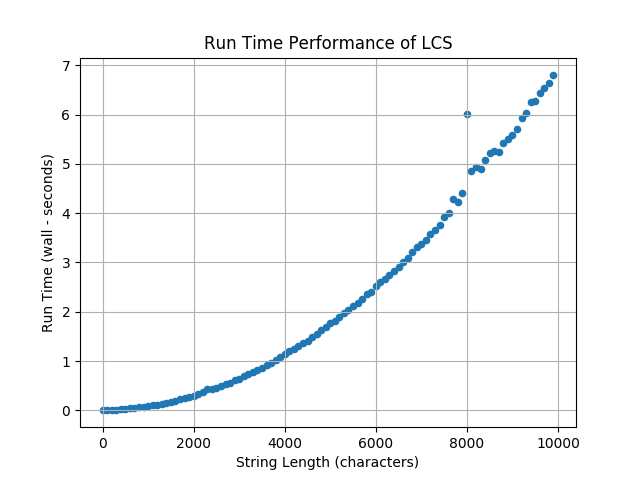
\includegraphics[width=10cm]{img/runtime_performance.png}
\end{figure}

The Python script can be run using the instructions in section B of the appendix.

\newpage